\date{29 января 2025}
\begin{theorem}
    Если $X$ хаусдорфово, а $A \subset X$ компактно, тогда $A$ замкнуто.
\end{theorem}
\begin{proof}
    Возьмём произвольную точку $x \in X\setminus A$ и $y\in A.$ Тогда существуют открытые окрестности $U(x,y)\ni x, V(x,y) \ni y$ такие, что $U(x,y) \cap V(x,y) = \emptyset.$ Так как $A$ компактно, то покроем конечным числом окрестностей. \[A \subset V(x, y_1) \cup \ldots \cup V(x,y_n).\] Тогда $U(x) \coloneq U(x,y_1) \cap \ldots \cap U(x, y_n)$ -- открытая окрестность точки $x$. Заметим, что $U(x) \subset X\setminus A$, значит $X \setminus A$ открыто, а $A$ замкнуто.
\end{proof}
\begin{theorem}
    Если $X$ компактно, а $f\colon X \to Y$ непрерывно, то $f(X)$ компактно.
\end{theorem}

\begin{proof}
    Без ограничения общности будем считать, что $Y = f(X)$. Пусть $\mathcal V = (V_\lambda)_{\lambda\in \Lambda}$ -- открытое покрытие $Y$. Тогда $f^* \mathcal V = (f^{-1}(V_{\lambda}))_{\lambda \in \Lambda}$ -- открытое покрытие для $X$. В силу компактности $X$, \[X = f^{-1}(V_{\lambda_1})\cup \ldots\cup f^{-1}(V_{\lambda_n}) \implies Y = V_{\lambda_1} \cup\ldots\cup V_{\lambda_n}.\]
\end{proof}

\begin{corollary}
    [Теорема Вейерштрасса] $f\colon [a;b]\to\R$ непрервыная функция, тогда $\exists \min f[a;b], \max f[a;b].$
\end{corollary}

\begin{theorem}
    Пусть $X$ компактно, $Y$ хаусдорфово, а $f\colon X \to Y$ -- непрерывная биекция, тогда $f$ -- гомеоморфизм.
\end{theorem}
\begin{proof}
    Нужно доказать, что $f(Z)$ замкнуто в $Y$, для любого замкнутого в $X$ множества $Z$. $Z$ замкнуто в компакте $X$, значит $Z$ компактно, тогда и $f(Z)$ компактно в хаусдорфовом $Y$, а значит $f(Z)$ замкнуто\footnote{Такое отображение, когда образ замкнутого множества замкнут и само отображение непрерывно, то оно называется \emph{замкнутым отображением.}}.
\end{proof}
\subsection{Критерий компактности в метрических пространствах}

\begin{theorem}
    $(X, \rho)$ -- секвенцально компактно, тогда оно полное\addtocounter{footnote}{1}\footnote{Заметим, что полнота -- свойство метрического пространства, нет смысла говорить о полном топологическом пространстве, только метрическом (Из \cref{def:fullness}).}.
\end{theorem}
\begin{proof}
    Пусть $(x_n)_{n\in\N}$ -- фундоментальная последовательность, тогда в силу секвенцальной компактности у нее есть сходящаяся подпоследовательность $x_{n_k}\to x$. Тогда и само $x_n \to x.$
\end{proof}
\begin{definition}
    [$\epsilon$-сеть]
    Подмножество $A\subset X$, где $(X, \rho)$ -- метрическое, называется $\epsilon$-сетью, если \[\forall x \in X \quad\exists a \in A \qquad \rho(a,x) < \epsilon.\]
\end{definition}
\begin{definition}
    [Вполне ограниченность]
    Говорят, что метрическое пространство $(X, \rho)$ вполне ограничено, если для него существует конечная $\epsilon$-сеть.
\end{definition}

\begin{proposition}
    Секвенцально компактное пространство вполне ограничено.
\end{proposition}
\begin{proof}
    Будем доказывать от противного, то есть существует $\epsilon$, что нет конечной сети. Возьмём какое-нибудь $x_1\in X$, а $x_n$ возьмём такое, что \[\rho(x_{n+1}, x_n) \geqslant \epsilon.\] Тогда это $\rho(x_n, x_m) \geqslant \epsilon \quad \forall n \neq m.$ Тогда у $(x_n)$ нет сходящейся подпоследовательности. 
\end{proof}
\begin{example}
    Пусть $C(X,Y) = \{f\colon X\to Y\such f \text{ непрерывно}\}$. Если $X, Y$ метрические, а $Y$ ограничено, то есть \[\exists c > 0 \quad \forall y_1, y_2 \in Y \quad \rho(y_1,y_2) < c. \] То в $C(X, Y)$ есть метрика \[\rho_c(f, g) \coloneq \sup_{x\in X}\rho(f(x), g(x)).\]
    Такая метрика называется равномерной.

    Тогда возьмём $C([0;1], [0;1])$ -- ограничено, но не вполне ограничено. Оно ограничено, потому что расстояние не больше 1. А не вполне ограничено, потому что не существует $\rfrac 1 2$-сети.

    \begin{figure}[h]
        \centering
        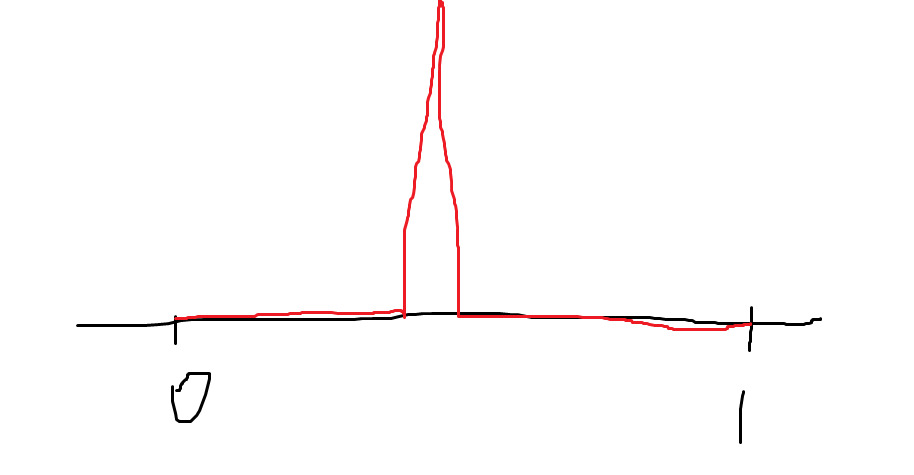
\includegraphics[width=0.7\linewidth]{graphics/spades-funcs.png}
        \caption{Если взять такое множество функций, то расстояние между такими всегда 1.}
    \end{figure}
\end{example}

\begin{theorem}
    Пусть Метрическое пространство $(X, \rho)$ тогда следующие условия эквивалентны: \begin{conditions}
        \item $X$ компактно;
        \item $X$ секвенцально компактно;
        \item $X$ полно и вполне ограничено.
    \end{conditions}
\end{theorem}
\begin{remark}
    Мы уже доказали (i) $\implies$ (ii) и (ii) $\implies$ (iii).
\end{remark}
\begin{lemma}
    $X$ вполне ограничено, тогда любое подмножетсов $Y \subset X$ тоже вполне ограничено.
\end{lemma}
\begin{proof}
    Пусть $M$ -- конечная $\rfrac \epsilon 2$-сеть в $X$, тогда $$\forall x \in M \leadsto a_x\in Y\quad\rho(x, a_x) < \frac \epsilon 2.$$
    Тогда $A = \{a_x\}$ конечно. Это $\epsilon$-сеть в $Y.$ \[\forall y \in Y \quad \exists x \in M\qquad \rho(x, y) < \frac \epsilon 2, \quad \rho(x, a_x) < \frac \epsilon 2 \implies \rho(y, a_x) < \epsilon.\]
\end{proof}